\section{Parallelisierung}
\label{sec:parallelpart}
  Im vorherigen Kapitel haben wir die Berechnung der Gravitationskräfte durch Interpolation approximiert. Dadurch konnten wir die Technik \hquad nutzen um den Rechenaufwand des Algorithmus zu 
  beschleunigen.
  Um die absolute Laufzeit aber noch weiter zu reduzieren sind wir an einer parallel arbeitende Variante dieses Algorithmus interessiert. In diesem Kapitel wird ein Ansatz vorgestellt.
  
  Ziel ist es, zunächst einen einfachen Algorithmus zu entwerfen. Daher beschränken wir uns auf Parallelisierung nach dem Message-Passing-Modell unter Verwendung von MPI. Wir können also 
  $p \in \N$ Prozesse starten. Jeder von diesen hat eine eindeutige $id \in \nullhaken{p-1}$ und seinen privaten Speicherbereich. Insbesondere ist in diesem Modell Shared-Memory ausgeschlossen. 
  Außerdem können die Prozesse miteinander kommunizieren um Daten auszutauschen. Die Menge der Prozesse wird im Folgen mit $\Proc$ bezeichnet.

  
  \subsection{Arbeitsverteilung}
  \label{sec:work}
    Damit wir von parallel arbeitenden Prozessen profitieren können, muss die Arbeit möglichst gleichmäßig auf diese Prozesse verteilt werden. Wir folgen, in modifizierter Variante, dem von 
    \citet{distrh2} vorgestellten Cluster-zentrierten Ansatz. 
    Dieser basiert auf dem Grundgedanken, dass für \vorruck ausschließlich Daten zwischen Vater- und Sohnclustern ausgetauscht werden müssen. Um möglichst viel Kommunikation zu sparen, ist es daher
    besonders effektiv, wenn möglichst viele Söhne durch den selben Prozess verarbeitet werden, wie der Vater. Besonders einfach wird das Verteilen der Cluster und das Loadbalancing, wenn wir $p$ als 
    Zweierpotenz $p = 2^q$ wählen. Da dann die Anzahl von Clustern in $T_\Omega^{(q)}$ gerade $p$ entspricht, können wir diese Ebene, zuzüglich der Sohncluster, optimal auf die Prozesse verteilen.
    Wir gehen im Folgenden immer von einer so gewählten Anzahl Prozesse aus.
    
    Um diesen Ansatz auf den Algorithmus zu übertragen, wird in der in \autoref{lst:init} aufgeführten init-Methode die globale Variable $\tcode{SPLIT_DEPTH} = log_2(p) = q$ gesetzt. 
    Außerdem bekommt die Datenstruktur \code{Cluster} einen weiteren Member: \code{int active}. In diesem  wird die $id$ des für dieses Cluster zuständigen Prozesses gespeichert.
    
    Zudem gibt es aber noch Cluster auf den Ebenen $T_\Omega^{<q} := T_\Omega^{(0)},\dots,T_\Omega^{(q-1)}$. Um ein Cluster $C \in T_\Omega^{<q}$ zu klassifizieren nutzt jeder Prozess $P \in \Proc$
    mit $id_P$ zwei Konstanten. Gilt für alle Nachfahren $\tilde C \in sons*(C)$ $C.\tcode{active} \neq id_P$  , wird der Member $C.\tcode{active}$ auf die \code{int}-Konstante \code{inactive} gesetzt. 
    Gibt es aber Nachfahren $\tilde C \in sons*(C)$ mit $C.\tcode{active} = id_P$, so wird der Member $C.\tcode{active}$ statt dessen auf die \code{int}-Konstante \code{semi_active} gesetzt. Inaktive
    Cluster werden während der \vorruck nicht weiter beachtet. 
    
    \begin{figure}[t]
    \begin{subfigure}{0.9\textwidth}
    \begin{lstlisting}[label=lst:parsetup, caption={Für die Verteilung der Cluster auf die Prozesse angepasste \code{_setup}-Methode.}]
void _setup(Cluster *c, int depth){
  if(depth == SPLIT_DEPTH){
    c->active = ++split_count;
  }

  if(depth < MAX_DEPTH){
    _setup_nonLeafCluster(c, depth);
  }

  if(c->active == semi_active){
    if(c->son[0]->active == inactive && c->son[1]->active == inactive){
      c->active = inactive;
    } else{
      if(c->son[0]->active != world.rank && c->son[0]->active != semi_active &&
	 c->son[1]->active != world.rank && c->son[1]->active != semi_active) {
	c->active = inactive;
      }
    }
  }
}
    \end{lstlisting}
    \end{subfigure}
    \end{figure}
    Um diese Einteilung vorzunehmen, wird vorrangig der Code der Methode \code{_setup(...)} (vgl. \autoref{lst:setup}) angepasst. 
    Zudem bekommt der Konstruktor \code{_new_bound_Cluster} einen neuen Parameter um den Member \code{active} aller Cluster zu initialisieren. Für die Konstruktion der Wurzel ist dieser auf
    \code{semi_active} gesetzt. Danach wird durch die Methode \code{_setup_nonLeafCluster(...)} immer der Wert des Vaters an die Söhne weitergegeben.
    Der angepasste Code der \code{_setup}-Methode ist in \autoref{lst:parsetup} aufgeführt.
    
    Zunächst wird überprüft, ob die \code{SPLIT_DEPTH} erreicht wurde. Ist dies der Fall wird der Member \code{active} auf 
    die $id$ des zuständigen Prozesses gesetzt. Dies geschieht einfach durch abzählen. Als nächstes folgt der bereits aus \autoref{lst:setup} bekannte Aufruf, der das Teilen in Sohncluster, das 
    Sortieren der \code{bodies} und die Rekursion beinhaltet. Der letzte Teil wird beim Abbau der Rekursion durchgeführt. Hier wird für eben die Cluster in $T_\Omega^{(<q)}$ überprüft ob diese 
    auf \code{semi-active} bleiben, oder, falls kein Nachfahre aktiv ist, der Member \code{active} auf \code{inactive} gesetzt wird.
    
    Die Idee der semi-aktiven Cluster beruht darauf, die Gestalt der Spalten- bzw. Zeilenmatrizen $V_\tau$ und $W_\sigma$ auszunutzen. Diese werden für Nicht-Blattcluster durch die Transfermatrizen 
    aus den Söhnen konstruiert (vgl. \autoref{sec:approxf}). Während der \vorw werden für ein solches Cluster $C_{semi} \in T_\Omega^{<q}$ die Ersatzmassen nur aus (semi-)aktiven Söhnen
    errechnet. Da diese Cluster für mehrere Prozesse als semi-aktiv gekennzeichnet sind, werden global betrachtet alle Söhne in der \vorw beachtet. Ist eines dieser Cluster Bestandteil
    eines zulässigen Blockes $b_0 = C_{semi} \times C$ oder $b1 = C \times C_{semi}$, so können die Prozesse ihre Berechnungen untereinander austauschen. Somit werden die Definitionen der Matrizen
    $V_\tau$ und $W_\sigma$ aus \autoref{eq:vtau} beziehungsweise \autoref{eq:wsigma} lediglich auf mehrere Prozesse verteilt und die Summation bei Bedarf aus den Teilergebnissen gebildet.
    
    Unter der Voraussetzung, dass alle notwendigen Information für jeden Prozess vorhanden sind, ist die einzige Anpassung der \koppl, dass sich die Auswertung auf (semi-)aktive
    Targetcluster beschränkt. Auch die \ruckw braucht sich lediglich auf (semi-)aktive Cluster beschränken.
    
    Letztlich verteilt sich die Arbeit durch diesen Ansatz sehr natürlich auf die Prozesse. In \autoref{fig:vertblock} ist dies veranschaulicht. Hier ist dies für einen Prozess $P$ mit $id_P = 1$ 
    und $p = 4$ dargestellt, welche Zuständigkeiten sich für die Blöcke des Blockbaumes aus der Aufteilung der Targetcluster ergeben.
    
    \begin{figure}[b]
      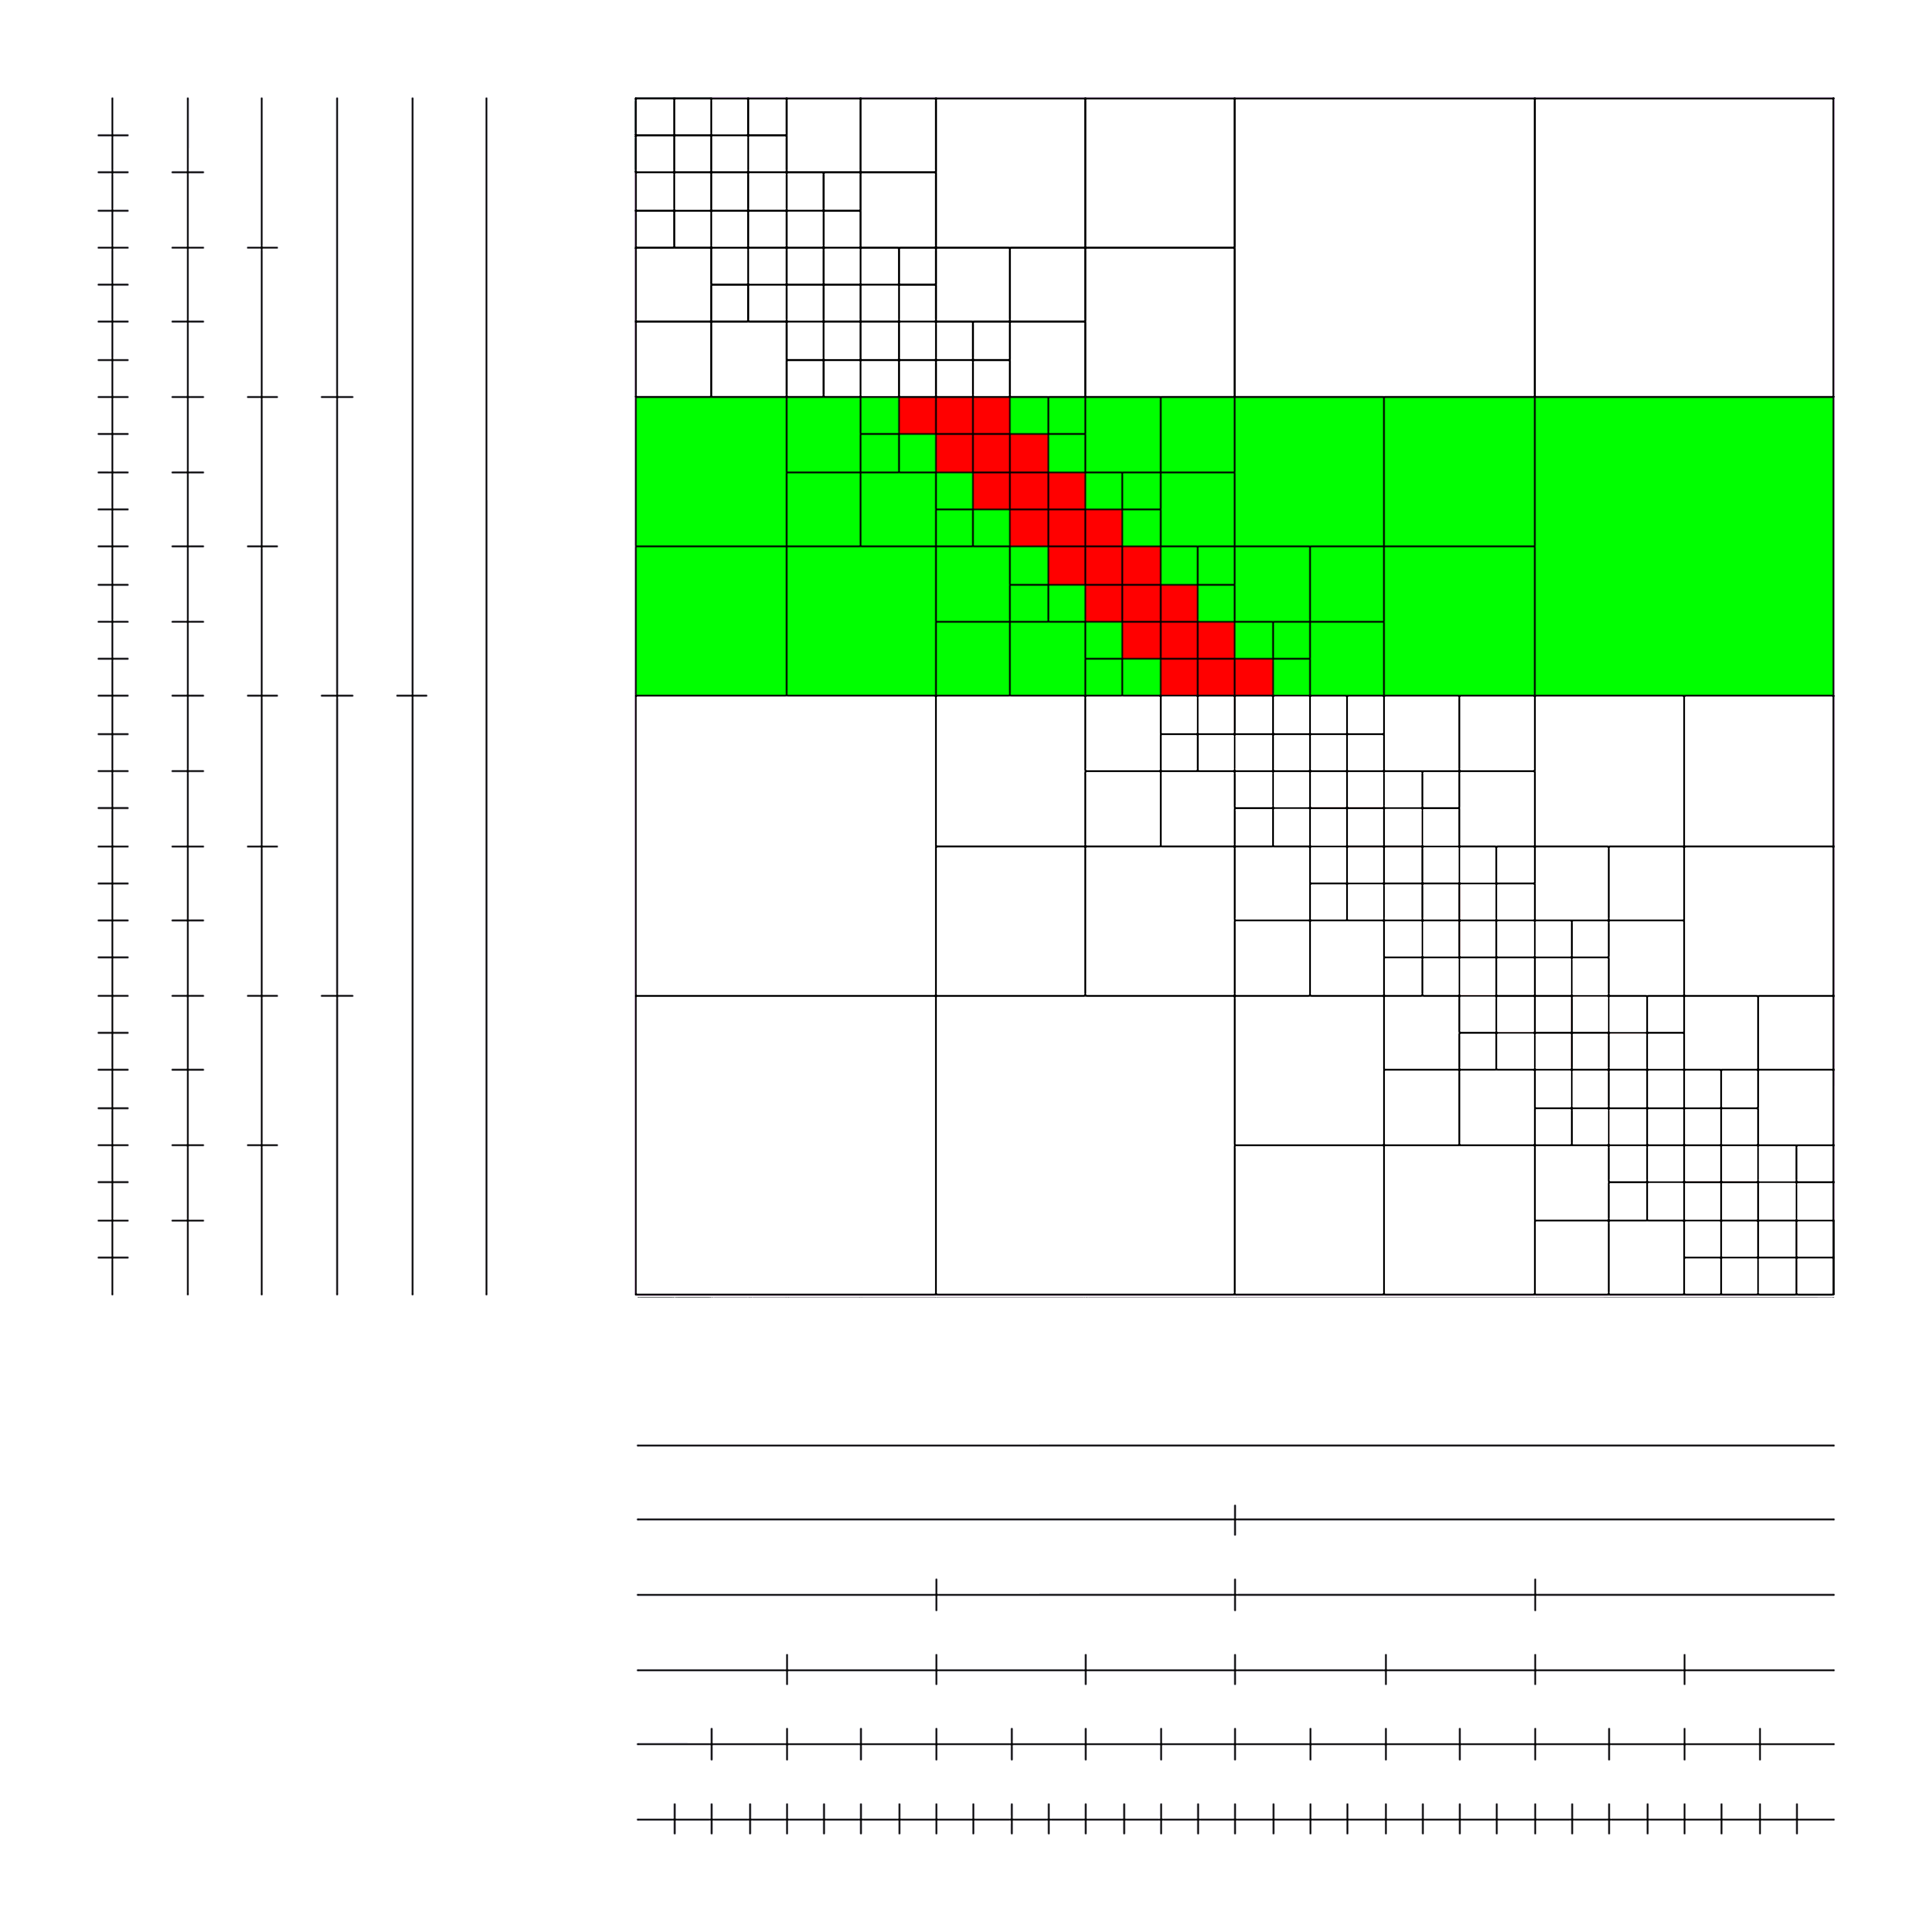
\includegraphics[width=0.77\textwidth]{img/verteilter_blockbaum.png}
      \caption{Für einen Prozess $P$ mit $id_P = 1$ und die Anzahl Prozesse $p = 4$ ist hier die Zuständigkeit des Prozesses $P$ für Blöcke eines Blockbaumes farbig dargestellt.
	       (Quelle: \citet{h2slides})}
      \label{fig:vertblock}
    \end{figure}

    \clearpage
  
  \subsection{Datenverteilung}
  \label{sec:data}
    \begin{figure}[b]
  \begin{subfigure}{0.9\textwidth}
    \begin{lstlisting}[label=lst:parconsttree, caption={Ausschnitt aus der parallelen Konstruktion des Clusterbaumes.}]
Cluster *constructClusterTree(bodies *b){
  [...]
  ////////////////////////////////////////////////////////
  // Sort the bodies; first locally, then globally.
  new_n  = preSort(root, 0);
  new_bs = new_bodies(new_n);
  alltoall_bodies(my_bs, send_count, send_displ, new_bs, recv_count, recv_displ);
  del_bodies(my_bs);
  my_bs = new_bs;
  //reset roots bodies*
  root->bodies = my_bs;
  root->n      = my_bs->n;
  
  //clean up
  
  [...]
}
    \end{lstlisting}
  \end{subfigure}
\end{figure}

\begin{figure}[t]
  \begin{subfigure}{0.9\textwidth}
    \begin{lstlisting}[label=lst:presort, caption={Diese Methode sortiert die lokalen \code{bodies} nach Prozesszugehörigkeit.}]
void preSort(Cluster *c, int depth){
    if(depth == SPLIT_DEPTH){
        c->active = ++split_count;
    
        //get count and start index of data to send to process #split_count
        send_count[split_count] = c->n;
        send_displ[split_count] = split_count == 0 ? 0 : send_displ[split_count - 1] + send_count[split_count - 1];
    
        //if the current knot is the active one: gather counts and displs from the other knots:
        MPI_Gather(&send_count[split_count], 1, MPI_INT, recv_count, 1, MPI_INT, split_count, MPI_COMM_WORLD);
        if(world.rank == c->active){
            new_n = 0;
            for(int i = 0; i < world.size; i++){
                recv_displ[i] = new_n;
                new_n        += recv_count[i];
            }
        }
        
    } 
    [...}] // Sortierung und rekursiver Aufruf
}
    \end{lstlisting}
  \end{subfigure}
\end{figure}

    Eine weitere grundlegenden Frage ist, wo welche Daten vorhanden sind. Ein Möglicher Ansatz wäre, dass jeder Prozess eine Kopie aller Daten hat. Doch selbst wenn das Gravitationsproblem kein all
    zu speicherhungriges ist, würde der Hauptspeicher bei 32 Prozessen auf einem Knoten\footnote{Dies entspricht den Spezifikationen der meisten Knoten des RZ-Clusters der Uni Kiel.}  sehr schnell 
    knapp werden. Außerdem sei an dieser Stelle an die weitere Skalierbarkeit des Problems erinnert (vgl. \autoref{sec:parrech}). Daher müssen die Daten über die Prozesse verteilt werden. 
    
    Da wir im vorigen Kapitel bereits beschrieben haben, wie die Arbeit effektiv verteilt werden kann, ist es nur naheliegend die Daten auf die gleiche Weise zu verteilen. Jeder Prozess soll also 
    genau die, zu seinen aktiven Clustern gehörenden, Teile der \code{bodies}-Struktur. Dies entspricht den hellblau gekennzeichneten Teilen des Clusterbaumes links in \autoref{fig:vertblock}.
    
    Weder bei reellen Daten, noch bei unseren zufällig generierten Testdaten, können wir davon ausgehen, dass diese nach Clustern sortiert vorliegen. Da ferner bei reellen Daten davon auszugehen
    ist, dass diese aus Platzgründen auch verteilt eingelesen werden müssen, generieren in unserem Programm auch alle Prozesse jeweils zufällige Testdaten. Es wäre möglich die Daten so verteilt
    zu belassen, wie sie generiert beziehungsweise eingelesen wurden. Jedoch wäre dann während der \vorruck eine große Menge an Kommunikation notwendig um diese entsprechend der Arbeitsverteilung
    durchzuführen. Daher ist es sinnvoll diese Daten einmal nach Prozesszugehörigkeit auszutauschen.
    
    Diese Kommunikation wird während der Konstruktion des Clusterbaumes vorgenommen. Der zugehörige Quellcode ist in \autoref{lst:parconsttree} und \autoref{lst:presort} aufgeführt.
    
    Die Methode \code{preSort(...)} sortiert die \code{bodies}, indem sie den Clusterbaum bis zur Ebene \code{SPLIT_DEPTH} konstruiert. In den Arrays \code{send_count[]} und \code{send_displ[]}
    merkt sich jeder Prozess, wie viele Elemente seiner \code{bodies} und ab welcher Position er an welchen anderen Prozess zu senden hat. Respektive werden in den Arrays \code{recv_count[]} 
    und \code{recv_displ[]} die Anzahlen und Pufferpositionen für die zu empfangenden Daten gespeichert. Diese werden über die Methode \code{MPI_Gather(...)} (vgl. \autoref{fig:kolkom} zwischen 
    den Prozessen ausgetauscht. So bekommt jeder Prozess von den anderen mitgeteilt, wie viele Elemente er von ihnen gesendet bekommen wird. Die Gesamtgröße der künftigen \code{bodies}-Memberarrays
    wird in \code{new_n} gespeichert.
    
    Der Datenaustausch findet über die Methode \code{MPI_Alltoallv(..)} (vgl. \autoref{fig:kolkom} und \autoref{lst:a2a}) statt. Diese führt mit Hilfe der zuvor konstruierten \code{count}- und 
    \code{displ}-Arrays gerade eine Transformation der ``Prozess-Daten-Matrix'' aus, wodurch jeder Prozess jedem anderen die zugehörigen Daten schickt und respektive von diesen erhält.
    Danach werden noch einige Variablen aktualisiert. 
    
    Schließlich wird der Clusterbaum wie gehabt vollständig bis zur Ebene \code{MAX_DEPTH} konstruiert. Hierfür sind die ausgetauschten Daten kaum notwendig, da die Konstruktion des Clusterbaumes
    durch mittige Teilung der Nicht-Blattcluster durchgeführt wird und zu diesem Zeitpunkt lediglich die Interpolationspunkte erstellt werden. Jedoch werden so gleich die korrekten Startindizes und
    Anzahlen in den Clustern gespeichert.
    